\documentclass{article}

\usepackage{fancyhdr}
\usepackage{graphicx}
\usepackage{extramarks}
\usepackage{enumerate}
\usepackage{amsmath}
\usepackage{hyperref}

\topmargin=-0.45in
\evensidemargin=0in
\oddsidemargin=0in
\textwidth=6.5in
\textheight=9.0in
\headsep=0.25in

\linespread{1.1}

\pagestyle{fancy}
\lhead{\paperAuthorName}
\chead{\paperTitle}
\rhead{\currentDate}
\lfoot{\teamName}
\renewcommand\headrulewidth{0.4pt}
\renewcommand\footrulewidth{0.4pt}

\setlength\parindent{0pt}

\graphicspath{ {images/} }

\newcommand{\enterSectionHeader}[1]{
\nobreak\extramarks{#1}{#1 continued on next page\ldots}\nobreak
\nobreak\extramarks{#1 (continued)}{#1 continued on next page\ldots}\nobreak
}

\newcommand{\exitSectionHeader}[1]{
\nobreak\extramarks{#1 (continued)}{#1 continued on next page\ldots}\nobreak
\nobreak\extramarks{#1}{}\nobreak
}

\setcounter{secnumdepth}{0}
\newcounter{customSectionCounter}

\newcommand{\customSectionName}{}
\newenvironment{customSection}[1][Section \arabic{customSectionCounter}]{
\stepcounter{customSectionCounter}
\renewcommand{\customSectionName}{#1}
\section{\customSectionName}
\enterSectionHeader{\customSectionName}
}{
\exitSectionHeader{\customSectionName}
}

\newcommand{\infoBox}[1]{
\noindent\framebox[\columnwidth][c]{\begin{minipage}{0.98\columnwidth}#1\end{minipage}}
}

\newcommand{\customSubSectionName}{}
\newenvironment{customSubSection}[1]{
\renewcommand{\customSubSectionName}{#1}
\subsection{\customSubSectionName}
\enterSectionHeader{\customSectionName\ [\customSubSectionName]}
}{
\enterSectionHeader{\customSectionName}
}

\newcommand{\paperTitle}{Address\ Book\ Design\ Document}
\newcommand{\paperAuthorName}{Zachary\ Trudo}
\newcommand{\teamName}{Team\ 666}
\newcommand{\currentDate}{2017-01-17}

% Title Page
\title{
\vspace{2in}
\textmd{\textbf{\paperTitle}}\\
\vspace{3in}
}

\author{\textbf{\paperAuthorName}}
\date{\currentDate}
\begin{document}

\maketitle

\newpage
\tableofcontents
\newpage

\begin{customSection}[Overview]
  Our goal is to create an Address Book meeting the requirements of the product
  specifications provided by Prof. Faulk. We will do this in three main phases:

  \begin{itemize}
    \item Minimum Viable Product (MVP) \\
      This will be the phase where we implement a minimial product that can
      perform the basic CRUD operations of an address book.
    \item GUI Implementation\\
      This will be the phase where we develop the GUI and link it to our MVP.
    \item Feature implementation\\
      This is the phase where we implement all features that are not CRUD related.
  \end{itemize}

  As a group we discussed what tools and software we'll be utilizing. To this
  end we have agreed upon the following:

  \begin{itemize}
    \item Programming Language\\
      Our main language will be Python 2.7.12. Python 2.7.12 was chosen due to
      the experience with the language on the team.
    \item GUI Framework\\
      The Tkinter package was chosen for our GUI framework. It was chosen due to
      its ease of use and alteration. We'll be iterating quickly and need a
      framework that supports efficient and rapid development.
    \item Save Format\\
      Our initial inclination for a save format was a mysql or mongo database.
      It was decided that a database requires too much overhead for such a
      simple application. We've decided to utilize the YAML file format in order
      to simplify the process of loading and saving. YAML corresponds directly
      with Python dictionary objects, and the PyYAML library makes loading,
      munging, and saving these objects easy and simple.
    \item Class Design Specifications\\
      Most class specifications will be done in UML. UML is ubiquitous and
      readily understood by all members of the team. 
  \end{itemize}
\end{customSection}

\newpage
\begin{customSection}[Minimum Viable Product (MVP)]
  The minimum viable product will be an command line address book that can perform
  the basic Create, Read, Update, Delete (CRUD) commands for an address book. This
  first step will provide us with a solid platform to link a GUI to in the future.
  \\
  Objects:
  \begin{itemize}
    \item Address \\
      This is the most basic object. Will contain all of the 'standard' address
      parameters, and functions for interacting with them.
      \begin{center}
          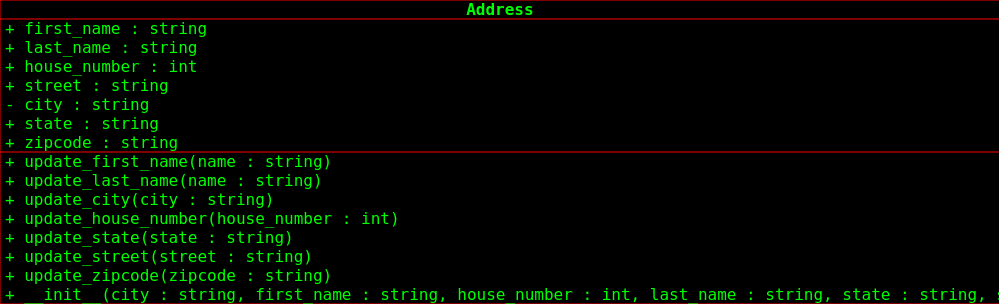
\includegraphics[width=\textwidth]{AddressUML}
      \end{center}
    \item AddressBook\\
      This is the book itself, it will handle updates to the book.
      \begin{center}
          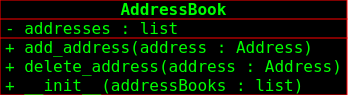
\includegraphics[width=\textwidth]{AddressBookUML}
      \end{center}
    \item FileOps\\
      This will be a static class that has the methods for interaction with the
      file system, producing address books from disk, and saving them to file
      using the YAML format. 
      \begin{center}
          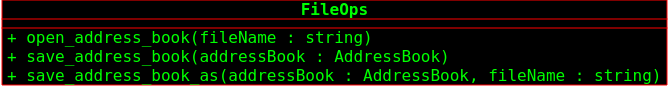
\includegraphics[width=\textwidth]{FileOPSUML}
      \end{center}
    \newpage
    \item basicCLI\\
      This will be our base for interaction with an AddressBook.

      Important design considerations:
      \begin{itemize}
        \item Undo/Redo functionality\\
          Undo and redo are important functions. We considered implementing
          either the
          \href{https://en.wikipedia.org/wiki/Memento_pattern}{Memento Pattern}
          or the \href{https://en.wikipedia.org/wiki/Command_pattern}{Command
          Pattern} but both were deemed too heavy handed for such a simple
          application.\\
          We've decided to go with a simple stateful approach, there will be a
          list called aBook, which will hold AddressBook objects. With every
          Create, Update, or Delete operation the AddressBook will be copied to
          the new state, and the new state will recieve the operation. The
          trade-off for the easier implementation  is that this is memory
          intensive, and will reduce the number of undo and redo operations that
          we can perform.
        \item Interface Layer\\
          The basicCLI should be entirely an interface layer with our three
          basic objects: Address, AddressBook, and FileOps. This will prove
          that we've created and designed a solid implementation, and ensure
          that our transition to a GUI interface will be simple and easy. To
          that end it is important that this implementation only ever interface
          with the underlying objects, rather than expanding or changing them.
          In example: Adding or deleting should utilize the add and delete
          functions provided by AddressBook. If the update function was being
          implemented here it would create a new Address object and replace the
          old one by deleting it and adding the new one.
      \end{itemize}
          
      Our basicCLI will support the following use cases:
      \begin{itemize}
        \item Create\\
          The ability to instantiate a new Address and place in the current
          AddressBook. The create() function will need to copy the current state
          to a new state, increment the current state to the new state, and then
          add the new address to the current state's AddressBook.
        \item Retrieve\\
          The ability to print to console an address from the current
          AddressBook. Will also return the Address object for updating and
          deleting. The retrieve() function will need to allow the user to
          select which contact they want from the list.
        \item Update\\
          The ability to alter the attributes of an Address. As the update
          function will look considerably different from the GUI implementation,
          it will not need to be implemented for the basicCLI.
        \item Delete\\
          The ability to remove an Address object from the current AddressBook.
          Will utilize the retrieve() function to get the specific address
          object that will need be removed from the AddressBook. Like the
          create() function, will need to copy the current state to a new state,
          increment the current state to the new state, and then remove the 
          address from the current state AddressBook.
        \item Save\\
          The ability to save to file the current AddressBook. Should just pass
          the current state's AddressBook to the FileOps save\_address\_book()
          function.
        \item Save As\\
          The ability to save to file the current AddressBook as a different
          filename. Should request a filename from the user, and pass the
          filename and current state's AddressBook to the FileOps
          save\_address\_book\_as() function. 
        \item Undo\\
          The ability to undo any of the create(), update(), or delete()
          actions. Should move the current state to the previous state, simply
          by decrementing the state and the undo count and incrementing the
          redo count. If we are at the earliest state, i.e. undo count is at
          zero - do nothing.
        \item Redo\\
          The ability to redo any undo action. Should move the current state to
          the next state, simply by incrementing the state and undo count, and
          decrementing the redo count. If we are at the latest state, i.e. redo
          count is at zero - do nothing.
      \end{itemize}
      \begin{center}
        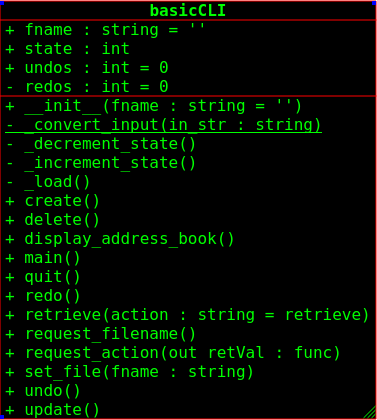
\includegraphics[width=\textwidth]{basicCLIUML}
      \end{center}
  \end{itemize}
\end{customSection}

\newpage
\begin{customSection}[Graphical User Interface implementation]
  The graphical user interface (GUI) will rely heavily on feedback from the
  customer. It is within this phase that we'll be able to present the customer
  with something they can interact with. Initially the GUI will support the same
  feature set as the basicCLI 
\end{customSection}

\end{document}
